\chapter{Results and discussion}
\label{sec:results}

\ifpdf
    \graphicspath{{Section4/Figs/Raster/}{Section4/Figs/PDF/}{Section4/Figs/}}
\else
    \graphicspath{{Section4/Figs/Vector/}{Section4/Figs/}}
\fi

\section{Comparison}

\subsection{Artificial Data}

Plotted in figures~\ref{fig:rotate} to~\ref{fig:translate}, and listed in tables~\ref{tab:rotation} to~\ref{tab:fracture} of Appendix~\ref{sec:appendix3}, are the timing and error (per pixel) values measured and calculated, respectively, averaged over three runs of each optical flow algorithm, so as to eliminate non-deterministic effects, for each of the affine transformations. The video sequences used varied from 480x480 pixels for a subsampling of 1, to 30x30 pixels for a subsampling of 16. The results shown in tables~\ref{tab:rotation} to~\ref{tab:fracture} in Appendix~\ref{sec:appendix3} are rounded to two decimal places, however the plots found in figures~\ref{fig:rotate} to~\ref{fig:translate} show the true values. The author was unable to construct the space dependent flow field required to calculate the accuracy of the fracture transformation, therefore only the timing information is included in table~\ref{tab:fracture}. However, it should be noted that the fracture transformation is effectively a translation.

\begin{figure}[h]
  \centering
  \makebox[\textwidth][c]{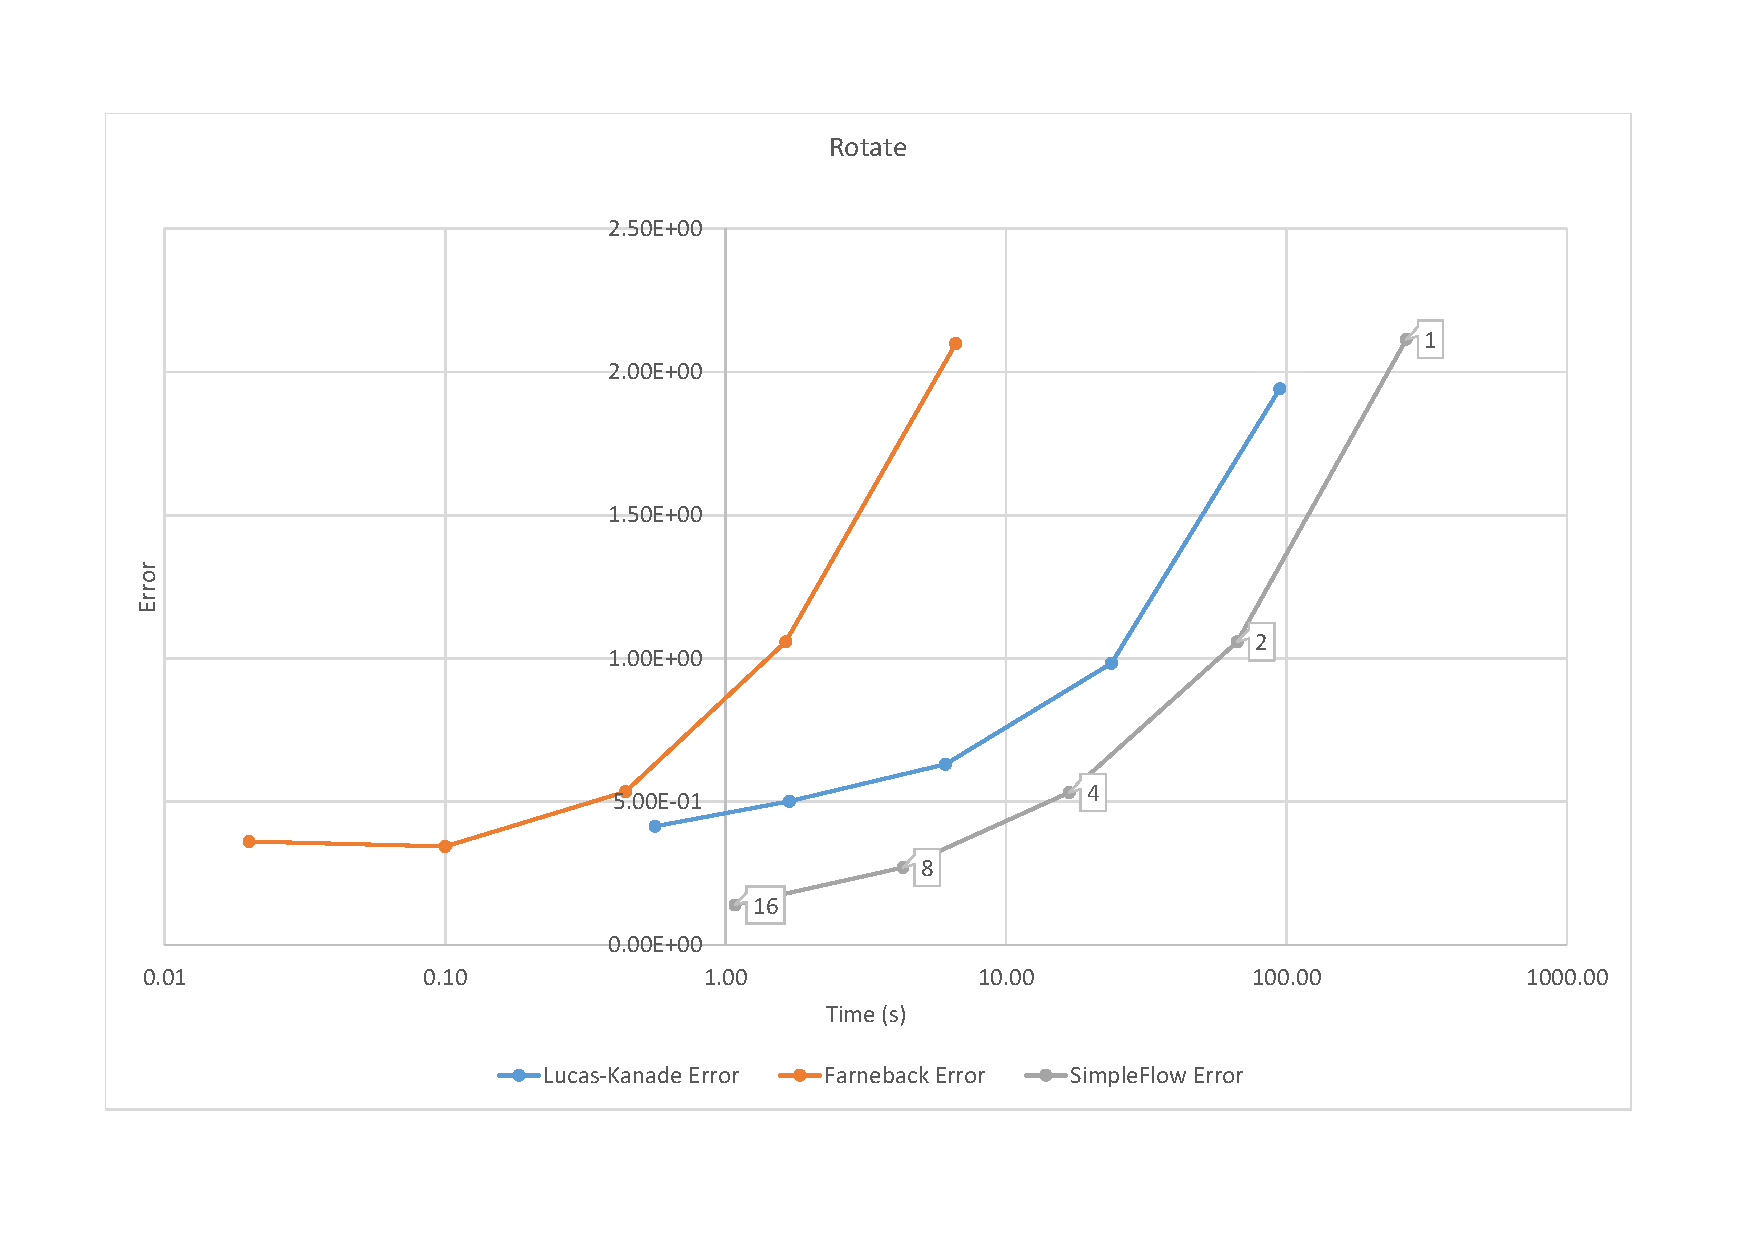
\includegraphics[width=1.2\textwidth]{rotate.pdf}}
  \caption{Rotate: Accuracy vs Speed}
  \label{fig:rotate}
\end{figure}

Firstly taking the results for the rotation transformation, plotted in figure~\ref{fig:rotate} and listed in table~\ref{tab:rotation} of Appendix~\ref{sec:appendix3}, it is plain to see that the error per pixel, and the processing time increases as the subsampling decreases, and conversely as the image size increases. For the higher subsampling in the rotation transformation the SimpleFlow algorithm has a lower error per pixel, however this is at the cost of a longer processing time per frame of video. As the sample sequences grow larger, the Farnebäck algorithm starts to show an advantage in the error per pixel. Consistently throughout the different frame sizes, the Lucas-Kanade method is the fastest.

\begin{figure}[h]
  \centering
  \makebox[\textwidth][c]{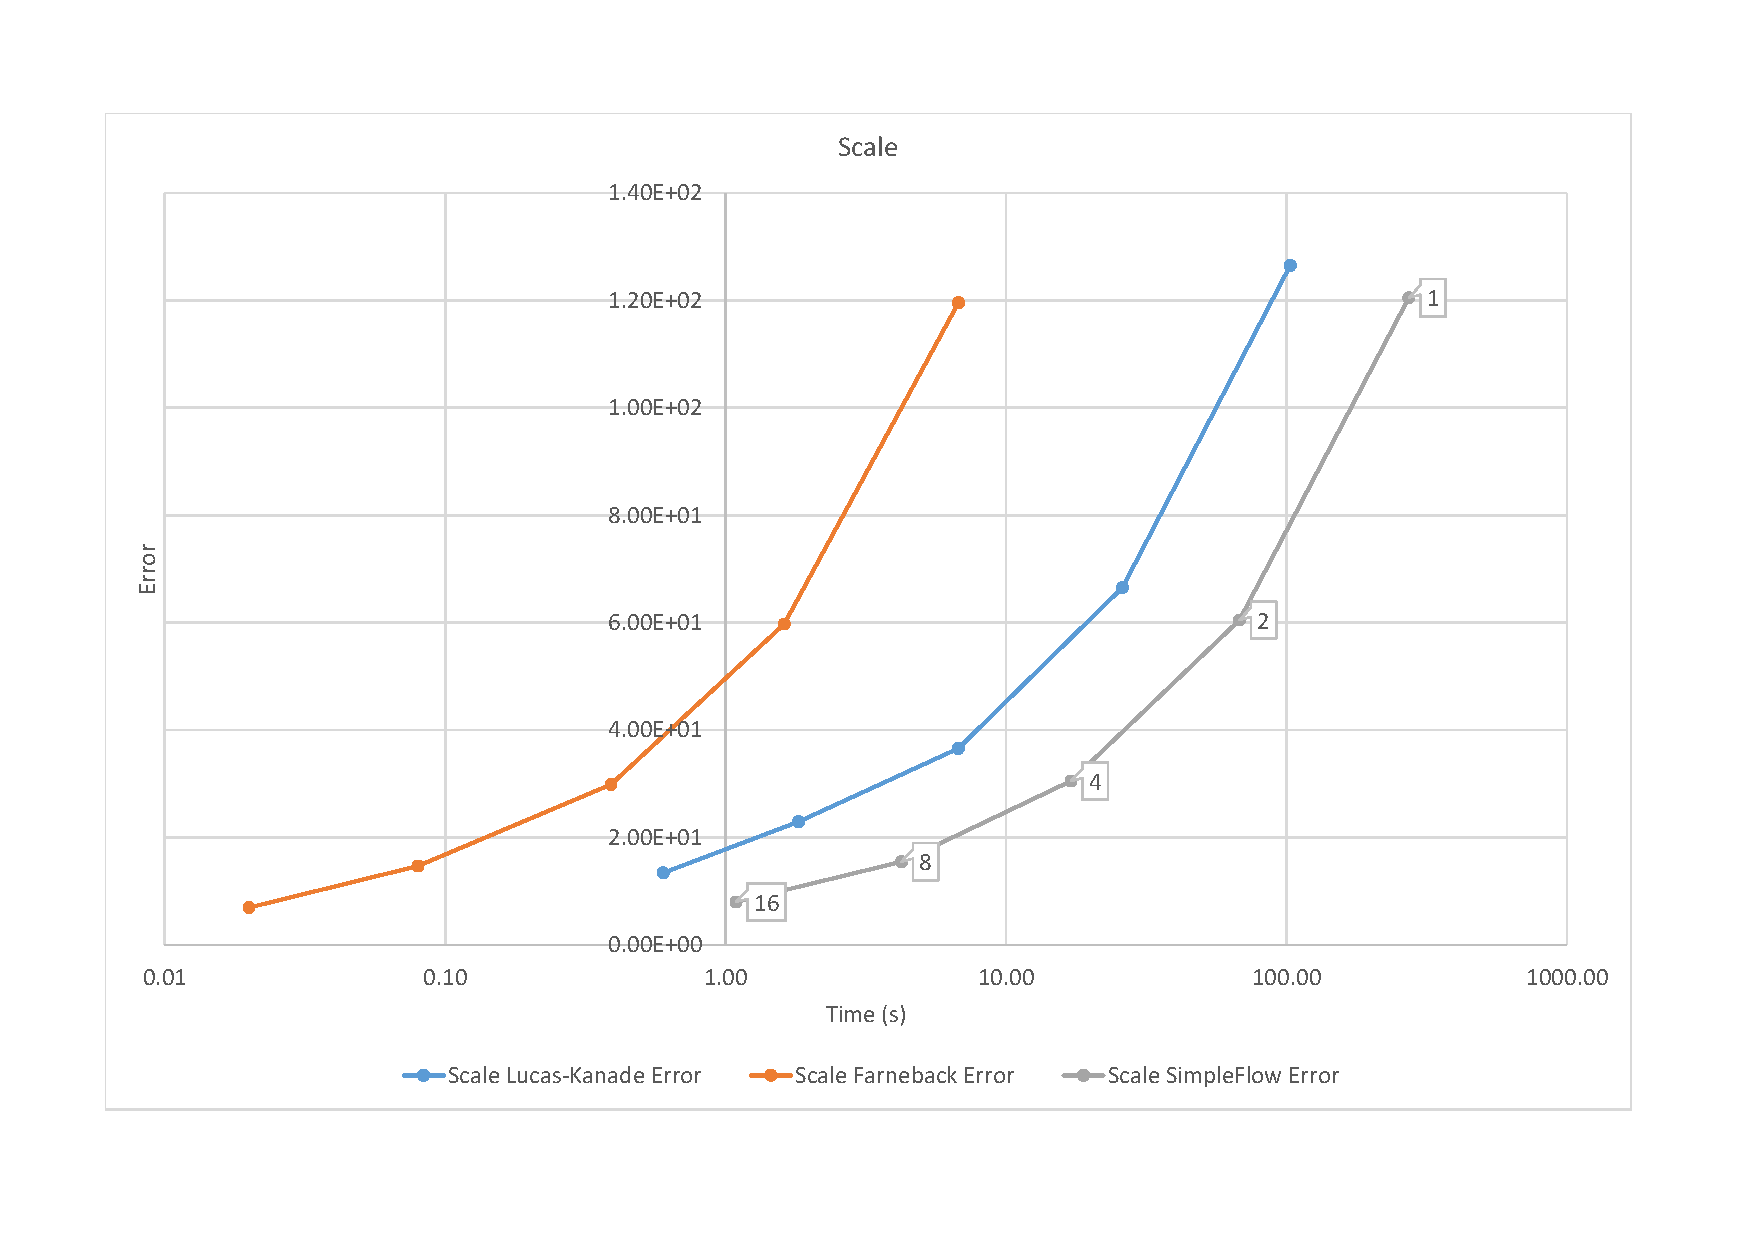
\includegraphics[width=1.2\textwidth]{scale.pdf}}
  \caption{Scale: Accuracy vs Speed}
  \label{fig:scaling}
\end{figure}

Looking at the results for the scaling transformation, plotted in figure~\ref{fig:scaling} and listed in table~\ref{tab:scale} of Appendix~\ref{sec:appendix3}, they are similar to those of the rotation transformation. That is to say, that the SimpleFlow algorithm has the longest processing time, while the Lucas-Kanade algorithm has the shortest processing time, with the Farnebäck algorithm lying somewhere in between. The main difference between scaling and rotation is that the Lucas-Kanade algorithm consistently wins out against the other two on accuracy.

\begin{figure}[h]
  \centering
  \makebox[\textwidth][c]{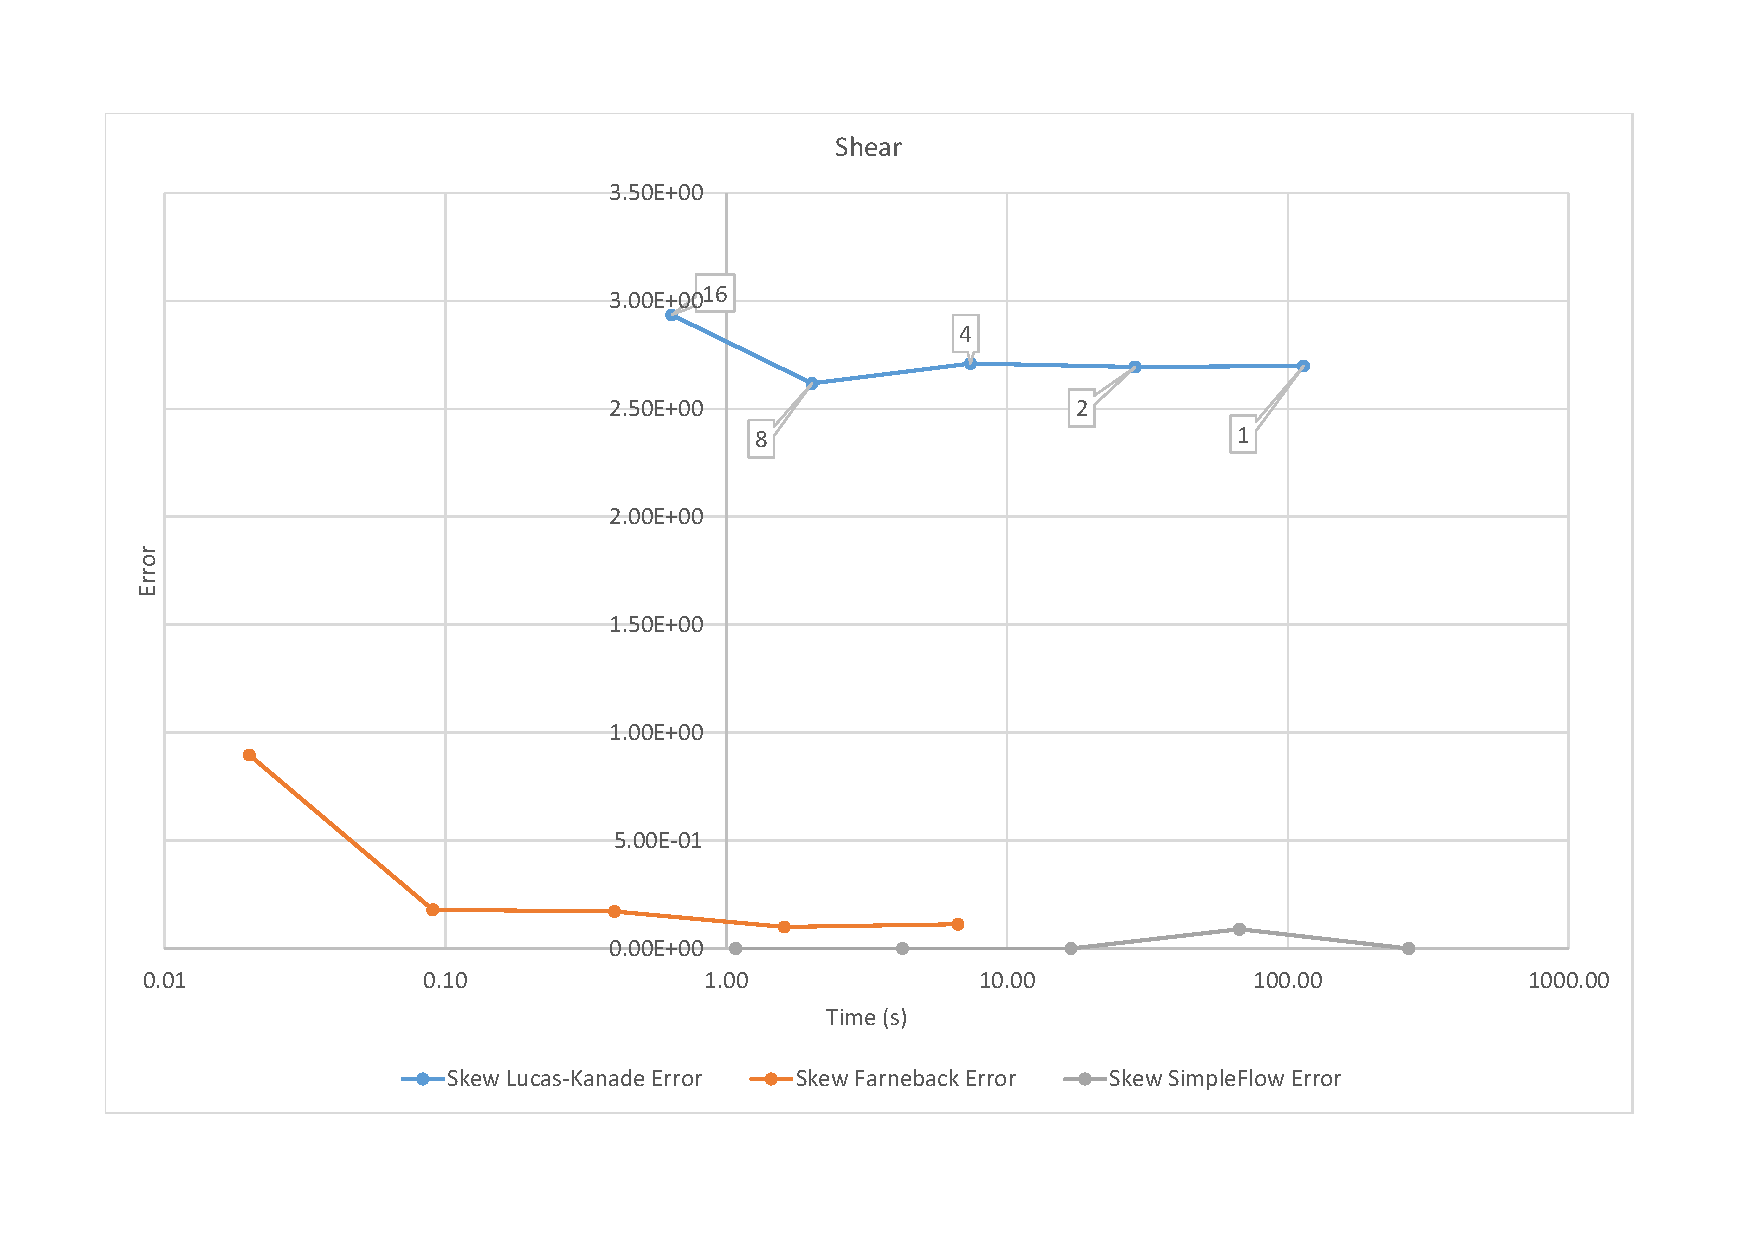
\includegraphics[width=1.2\textwidth]{shear.pdf}}
  \caption{Shear: Accuracy vs Speed}
  \label{fig:shear}
\end{figure}

Looking at the results for the shear transformation, plotted in figure~\ref{fig:shear} and listed in table~\ref{tab:shear} of Appendix~\ref{sec:appendix3}, they present a different view to either of the two transformations previously mentioned. All three algorithms have approximately uniform error across all subsampling amounts, however the processing time increases as the subsampling decreases, or conversely, as the frame size increases. SimpleFlow presents the lowest error per pixel of all three optical flow algorithms, however on larger images it has the longest processing time per frame. The other two algorithms present higher errors per pixel, however the Farnebäck algorithm appears to be very efficient at processing shear transformations compared to the other two algorithms.

\begin{figure}[h]
  \centering
  \makebox[\textwidth][c]{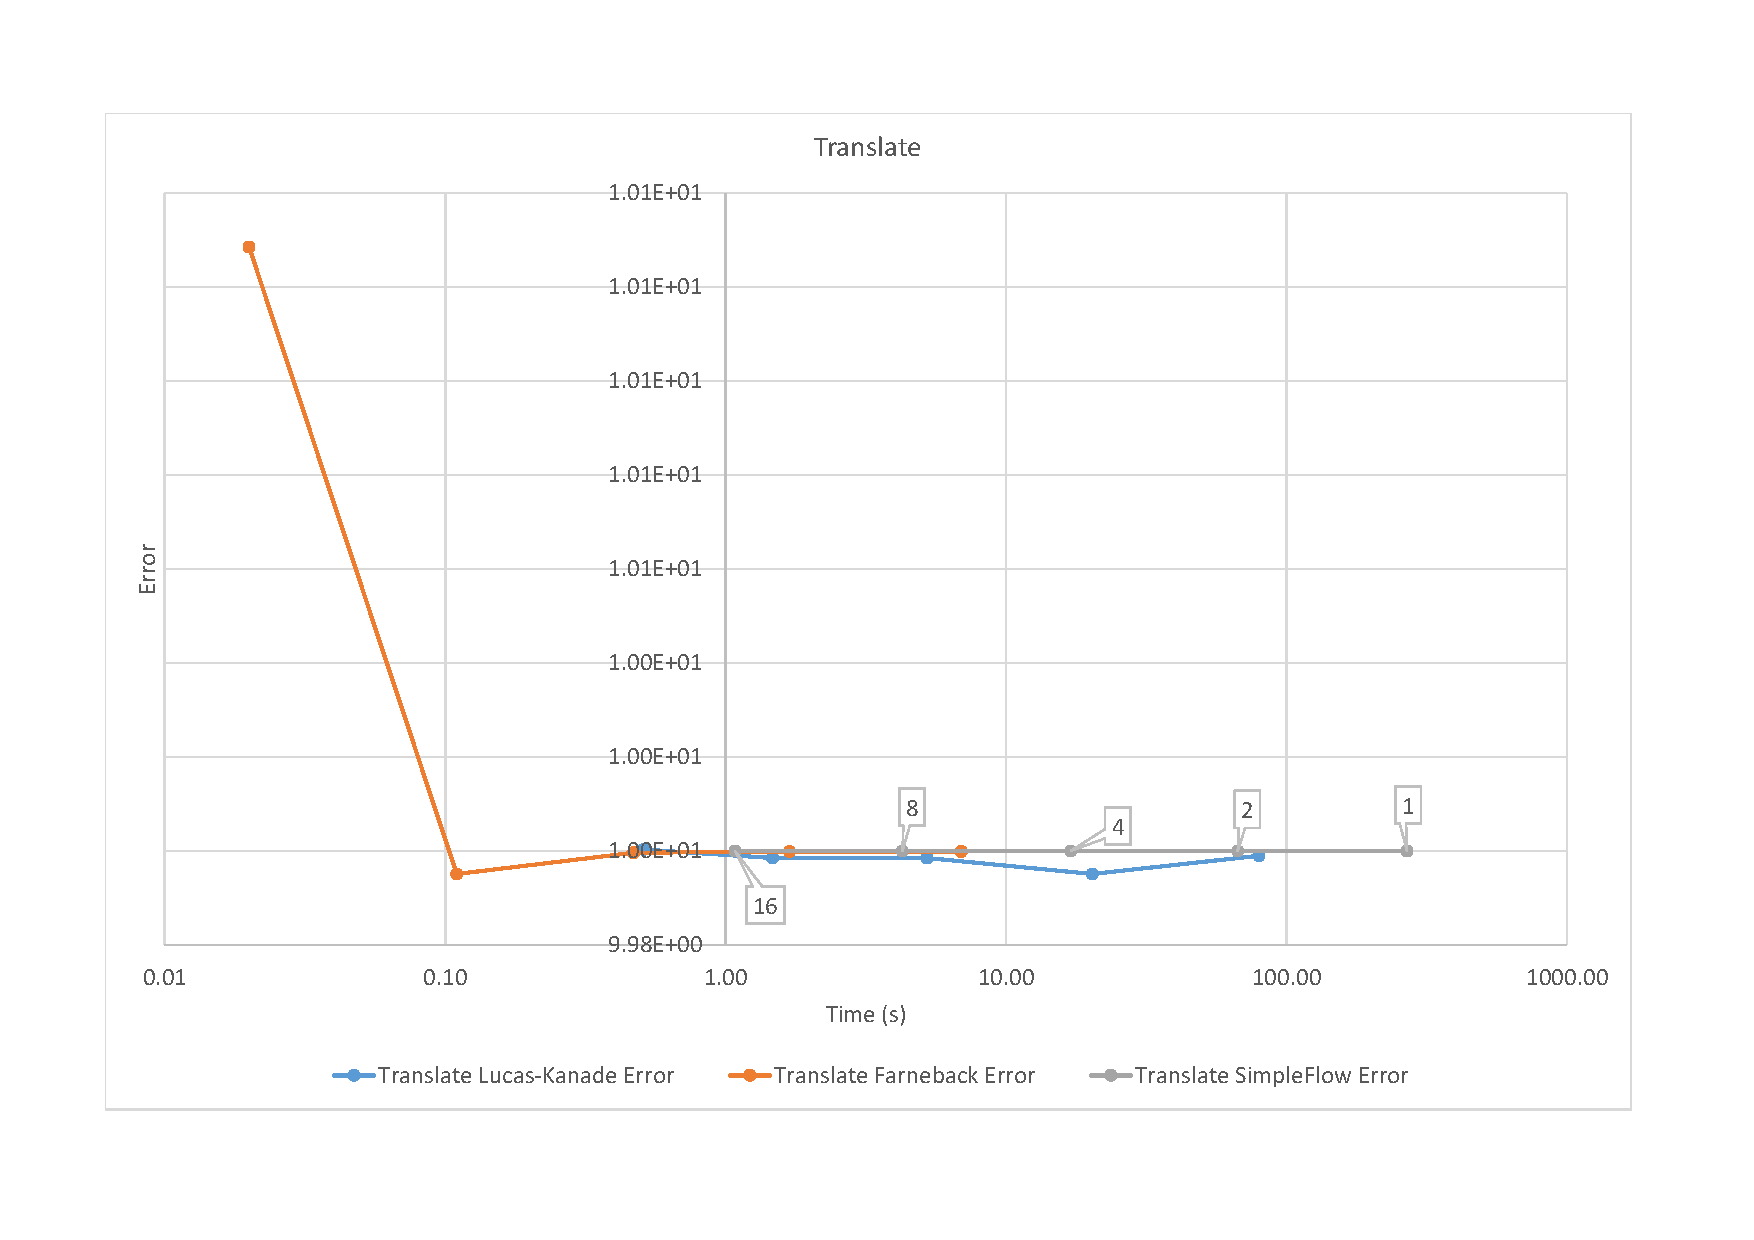
\includegraphics[width=1.2\textwidth]{translate}}
  \caption{Translate: Accuracy vs Speed}
  \label{fig:translate}
\end{figure}

Looking at the results for the translate transformation, plotted in figure~\ref{fig:translate} and listed in table~\ref{tab:translate} and  of Appendix~\ref{sec:appendix3}, all three optical flow algorithms appear to produce approximately the same error per pixel across all amounts of subsampling. The slight exception is the Farnebäck algorithm, which slightly outperforms the other two. The SimpleFlow algorithm is once again shown to be the slowest algorithm, while the Lucas-Kanade algorithm is shown to be the quickest.

\begin{table}[htbp]
  \centering
  \begin{tabular}{r|rr|rr|rr}
    \toprule
    & \multicolumn{2}{c}{Lucas-Kanade} & \multicolumn{2}{c}{Farnebäck} & \multicolumn{2}{c}{SimpleFlow} \\
    \midrule
    Subsampling & Time (s) & Error & Time (s) & Error & Time (s) & Error \\
    \midrule
    1 & 74.60 &       & 6.37  &       & 267.70 &  \\
    2 & 18.73 &       & 1.61  &       & 67.18 &  \\
    4 & 4.90  &       & 0.44  &       & 16.92 &  \\
    8 & 1.39  &       & 0.10  &       & 4.31  &  \\
    16 & 0.49  &       & 0.02  &       & 1.09  &  \\
    \bottomrule
  \end{tabular}
  \caption{Fracture}
  \label{tab:fracture}
\end{table}

The author was unable to construct the space dependent flow field required to calculate the accuracy of the fracture transformation, therefore only the timing information is included in table~\ref{tab:fracture} for posterity.
 
Looking at the results as a whole, it is clear when choosing an optical flow algorithm to be used on a dataset there are trade-offs that need to be made. When looking at an online, realtime application, the Farnebäck optical flow algorithm should be the forerunner due to the consistent low processing time across all different levels of subsampling, as well as all different affine transformations. The disadvantage to this choice is the lower accuracy obtained. If the application requires high accuracy, and is an offline processing application, then the SimpleFlow optical flow algorithm provides high accuracy, but this comes at the cost of a long processing time. As noted before, the SimpleFlow algorithm is highly parallelisable, and is designed for GPU acceleration. On future versions of the Raspberry Pi, or on workstation PCs, which may have these features, the SimpleFlow algorithm should perform better than on a single core, low clock CPU. If the application requires online, but only near-realtime processing, then the Lucas-Kanade optical flow algorithm is a strong candidate. Its processing time is consistently between that of the Farnebäck and SimpleFlow algorithms, and while is does provide good accuracy, its accuracy is not consistent across all affine transformations. As stated in section~\ref{sec:theory}, \nameref{sec:theory}, optical flow methods introduce an additional constrain to enable estimation of the optical flow, and the assumptions or approximations used in each optical flow algorithm may have an effect on how accurate it is with different affine transformations.
 
\subsection{Real World Data}

As there is no accurate, prior knowledge of the vector flow field, these datasets can only be used to compare the three optical flow algorithms for speed quantitatively, and for accuracy qualitatively. Table~\ref{tab:realworld} shows the processing time for the two data sets provided by Dr Alexandre Kabla~\cite{harris2012characterizing}, a lecturer and researcher in CUED, and Mustafa Kamal, A PhD student in the Hopkinson Lab.
 
\begin{table}[htbp]
 \centering
 \begin{tabular}{r|rrr}
   \toprule
   & \multicolumn{3}{c}{Processing Time (s)} \\
   Frame Size (MP) & Lucas-Kanade &  Farnebäck &  SimpleFlow \\
   \midrule
   0.3   & 1.39  & 3.45  & 418 \\
   0.7   & 2.40  & 6.65  & 718 \\
   \bottomrule
  \end{tabular}
  \caption{Real Word Data}
  \label{tab:realworld}
\end{table}

It is apparent that the Lucas-Kanade optical flow algorithm is the fastest, this is most likely due to it being a sparse method. Following closely is the Farnebäck algorithm, and lastly the SimpleFlow algorithm. The SimpleFlow algorithm's poor speed performance is most likely due to it being designed to be a highly parallelisable, GPU accelerated algorithm. As the Raspberry Pi has a single core ARM CPU, and its GPU is not able to utilised for CUDA or OpenCL accelerated processing, it should not be surprising that the SimpleFlow algorithm performs poorly on the Raspberry Pi. This shows that when the Lucas-Kanade algorithm is used as a true sparse optical flow algorithm, it has the ability to outperform the Farnebäck and SimpleFlow algorithms, as opposed to being forced to be a dense optical flow algorithm, in the previous section, when it operates more slowly than the Farnebäck algorithm.

\begin{figure}[h!]
  \centering
  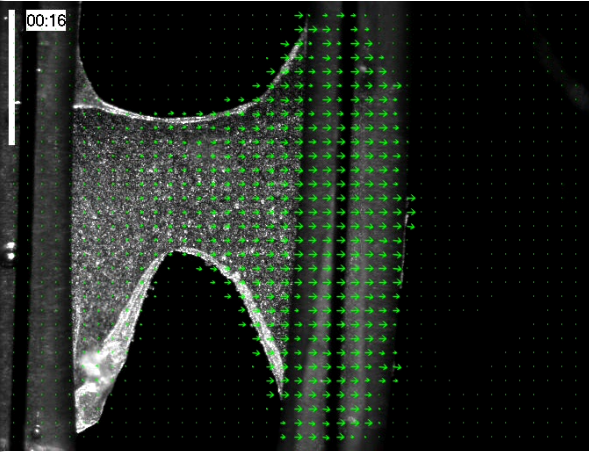
\includegraphics[width=.6\textwidth]{quiver}
  \caption{Vector flow depicted on top of the video frame}
  \label{fig:quiver}
\end{figure}

In order to aid the visualisation of the vector field of the real world data, and therefore assess the qualitative accuracy of the optical flow algorithms, the vectors calculated from the optical flow methods are drawn on top of each frame of the video. The method used is similar to the MATLAB function \verb|quiver| in that it automatically scales the arrows depending on the magnitude of the vector. An example of the output can be seen in figure~\ref{fig:quiver}.

\begin{figure}[htbp!]
  \centering
  \begin{subfigure}[b]{0.45\textwidth}
    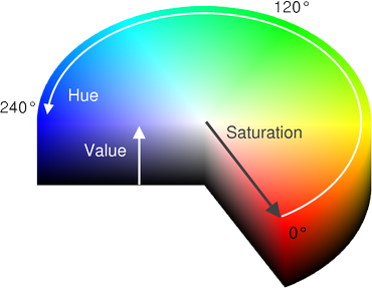
\includegraphics[width=\textwidth]{HSV}
    \caption{Mapping of vectors to HSV colour space}
    \label{fig:hsv}
  \end{subfigure}
  \begin{subfigure}[b]{0.45\textwidth}
    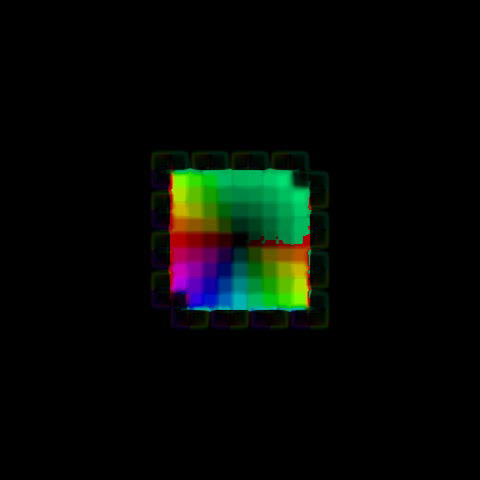
\includegraphics[width=\textwidth]{colour}
    \caption{Colour mapping of a scaling}
    \label{fig:colourmap}
  \end{subfigure}
  \caption{Mapping the vector field to the HSV colour space}
  \label{fig:colour}
\end{figure}

The vector field can also be represented using a colour map. This is achieved by converting the Cartesian vector coordinates into polar coordinates which are then mapped onto the HSV colour space as: Hue = Angle, Saturation = 255, Value = Magnitude. This can be seen in figure~\ref{fig:colour} which depicts the colour mapping of the scaling operation from the artificial dataset. This visualisation method is very useful to gain a quick insight into the apparent motion of the object being observed, without having to further process the vector field from the optical flow algorithm. It should be noted that while this colour mapping is possible for all optical flow algorithms, it is most effective for dense optical flow algorithms. Therefore the Lucas-Kanade algorithm will be required to track all points to achieve a similar output to that of the Farnebäck and SimpleFlow algorithms.

\section{Mechanical Testing}

One of the other goals of this project was the integrate with other projects in the OpenLabTools initiative. One such project was a mechanical testing rig designed and built by Josie Hughes. It allows for tensile testing of materials, and is based around the Arduino, an open-source electronics prototyping platform. Therefore two programs were authored in order to demonstrate online and offline processing. The online processing program makes use of the Lucas-Kanade algorithm due to the ability to select points to be tracked, however it also features an automatic point selector which calculates the minimal eigenvalue of gradient matrices for corner detection. The help text for the online processing program is as follows

\begin{verbatim}
Hot keys:
ESC - quit the program
r - auto-initialize tracking
c - delete all the points
n - switch the "night" mode on/off
To add/remove a feature point click it
\end{verbatim}

Night mode only shows the vector arrows of the flow field over a black background, in an effort to make the optical flow of the points being tracked easier to view. The source code for the online processing program can be seen in full online~\cite{github}

The offline processing program uses the Farnebäck algorithm, and while it is a dense optical flow algorithm, processing time is not as important as we are processing offline. Images for the offline method can be obtained by using the \verb|raspistill| command line program~\cite{raspistill}. The help text for the offline processing program is as follows:

\begin{verbatim}
Usage: ./offline frame1 frame2 output...
\end{verbatim}

The source code for the online processing program can be seen in full online~\cite{github}

In order to test the functionality of the programs, a tensile test of a rubber band was setup. A frame from the testing sequence with the flow field overlaid can be seen in figure~\ref{fig:instron}. This image shows that there is some optical flow occurring in the sequence, however the algorithm, in this example Farnebäck optical flow as this was processed offline, has mostly focused on the motion of the rig holding the rubber band in place. This is most likely due to the high contrast between the rig, and the background. Better framing of the rubber band in the sequence, and a high contrast background behind the mechanical testing rig should eliminate this problem.

\begin{figure}[h]
  \centering
  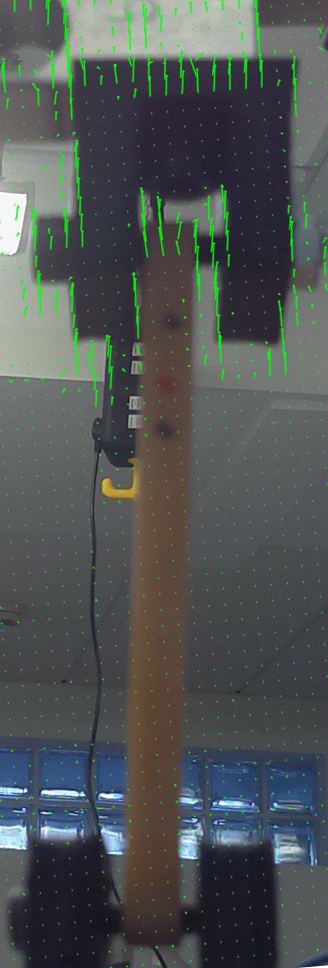
\includegraphics[height=.5\textheight]{output}
  \caption{Tensile test of rubber band}
  \label{fig:instron}
\end{figure}